In what follows we will be re-doing the numerical experiments presented in 
Zhong et al. \cite{zhgh93}.

The first benchmark showcases a unit square domain with free slip 
boundary conditions prescribed on all sides.
The resolution is fixed to 64x64 $Q_1 \times P_0$ elements. 
The flow is isoviscous and the buoyancy force is given by 
\begin{eqnarray}
f_x &=& 0 \nonumber\\
f_y &=& \rho \alpha T(x,y) \nonumber
\end{eqnarray}
with the temperature field given by 
\[
T(x,y) = \cos(kx) \delta(y-y_0)
\]
where $k=2\pi/\lambda$ and $\lambda$ is a wavelength, 
and $y_0$ represents the location of the buoyancy.

One can prove (\cite{zhgh93} and refs. therein) that 
there is an analytic solution for the surface stress $\sigma_{zz}$:
\[
\frac{\sigma_{yy}}{\rho \alpha g} =
\frac{\cos (kx)}{\sinh^2(k)}
\left[
k(1-y_0)\sinh(k) \cosh(ky_0)-k \sinh(k(1-y_0))
+\sinh(k) \sinh(ky_0)
\right]
\]

{\bf Remark}: This is suspicious since $\rho \alpha g$ does not have the 
dimensions of a stress! Instead we shall use $\rho \alpha g h$, and choosing 
where $h$ is the element size.

\begin{center}
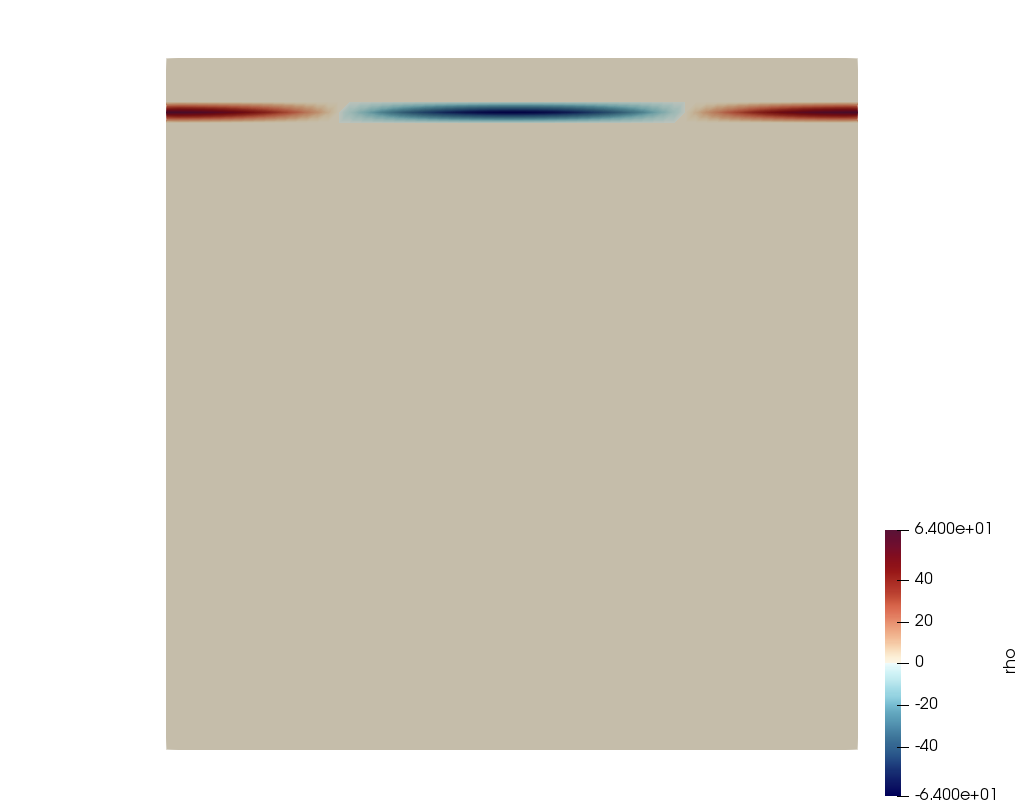
\includegraphics[width=6cm]{python_codes/fieldstone_27/rho}\\
density field for $y_0=59/64$
\end{center}

We choose $\rho \alpha = 64$, $\eta=1$, $g_y=-1$ (note that in this case the 
normalising coefficient of the stress is exactly 1 so it is not implemented).
$\lambda=1$ is set to 1 and we explore $y_0 = \frac{63}{64},\frac{62}{64},\frac{59}{64}$.
Zhong et al. report the following measurements
\footnote{The paper says 60/64 in the last column but it is in fact 59/64}
 at $x=0$:

\begin{center}
\begin{tabular}{l||lll}
\hline
Method             & $y_0=63/64$ & $y_0=62/64$ &  $y_0=59/64$ \\ 
\hline
\hline
Analytic solution                   & 0.995476 & 0.983053  &  0.912506 \\
Pressure smoothing                  & 1.15974  & 1.06498   &  0.911109 \\
CBF                                 & 0.994236 & 0.982116  &  0.912157 \\
\hline
fieldstone: elemental               & 0.824554 & 0.978744  & 0.909574 \\
fieldstone: nodal (C$\rightarrow$N) & 0.824554 & 0.978744  & 0.909574 \\
\hline
\end{tabular}
\end{center}

The $yy$ component of the stress tensor is simply given by
\[
\sigma_{yy} = -p + 2 \eta \dot{\epsilon}_{yy}
\]
and we start with trivial measurements in the elements 
forming the top row of the mesh (pressure is by definition elemental, and strain rate
components are computed in the middle of each element). 

\begin{center}
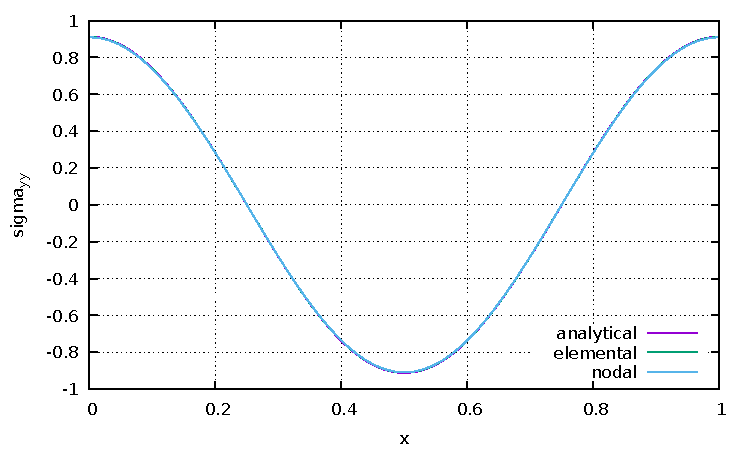
\includegraphics[width=5cm]{python_codes/fieldstone_27/results/59_64/sigmazz.pdf}
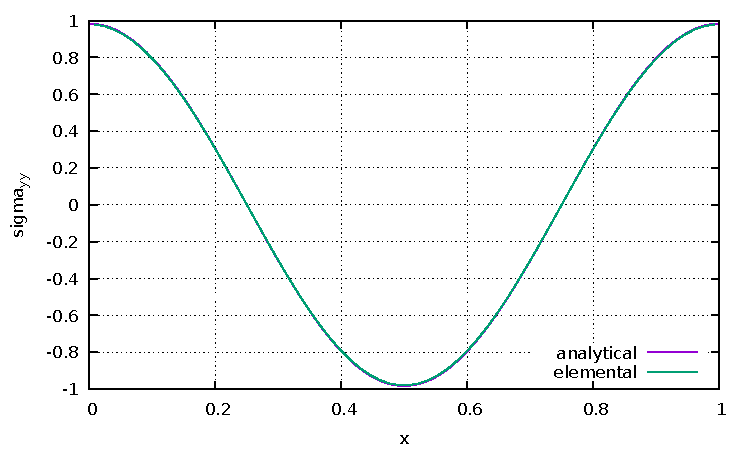
\includegraphics[width=5cm]{python_codes/fieldstone_27/results/62_64/sigmazz.pdf}
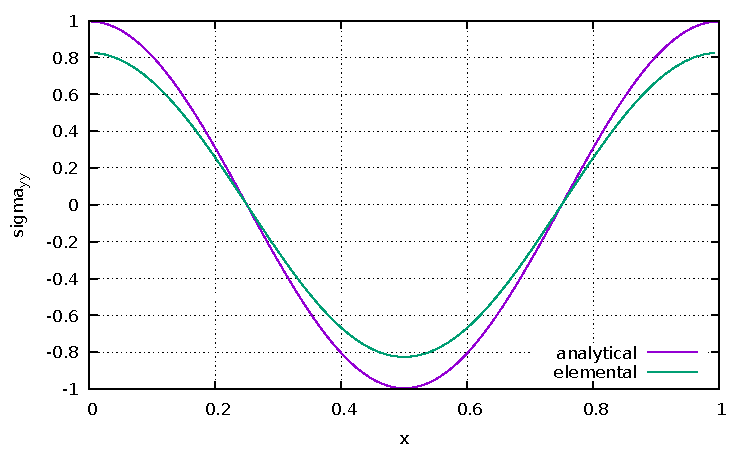
\includegraphics[width=5cm]{python_codes/fieldstone_27/results/63_64/sigmazz.pdf}
\end{center}






\fbox{
\parbox{10cm}{{\bf features}
\begin{itemize}
\item $Q_1\times P_0$ element \index{$Q_1 \times P_0$}
\item incompressible flow \index{incompressible flow}
\item mixed formulation \index{mixed formulation}
\item isothermal \index{isothermal}
\item isoviscous \index{isoviscous}
\item analytical solution \index{analytical solution}
\item pressure smoothing \index{pressure smoothing} 
\item consistent boundary flux \index{CBF}
\end{itemize}
}}

